\subsection*{Example}
Consider a viscous liquid in steady state that is in a downward motion in a narrow channel. 
\begin{figure}[h]
    \centering
    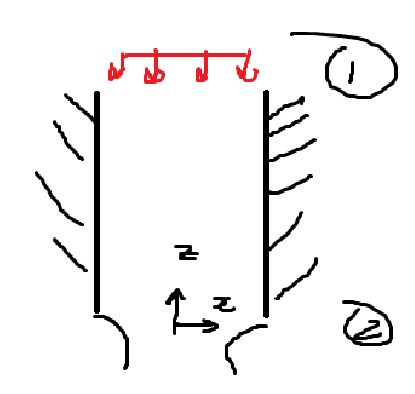
\includegraphics[width=0.2\textwidth]{Lecture Number/Figures/example 1, Feb 1, 2024.png}
    \caption{Viscous Liquid in a Narrow Channel}
    \label{fig:Example 1, Feb 1, 2024}
\end{figure}
\begin{enumerate}[label=(\alph*)]
    \item Write the full Navier-Stokes equations in the z-direction with body forces using index notation.
    \item Simplify the obtained equation from (a) for a fully-developed, 2D, steady flow with cartesian viscosity across the channel width. 
\end{enumerate}

(a) We write the general form of the Navier-Stokes equation:
\begin{align*}
    \frac{\partial}{\partial t} (\rho u_i) + \frac{\partial}{\partial x_j} (\rho u_i u_j) = -\frac{\partial P}{\partial x_i} + \frac{\partial}{\partial x_j} \left(\mu \left(\frac{\partial u_i}{\partial x_j} + \frac{\partial u_j}{\partial x_i}\right)\right) - \frac{\partial}{\partial x_i} \left(\frac{2}{3}\mu \frac{\partial u_k}{\partial x_k}\right) + \rho b_i
\end{align*}
in the z-dir, $i = 3$:
\begin{align*}
    \boxed{\partial_{t} (\rho w) + \partial_{j} (\rho w u_j) = -\partial_{z} P + \partial_{j} \left(\mu \left(\partial_{j} w + \partial_{i} u_j\right)\right) - \partial_{z} \left(\frac{2}{3}\mu \partial_{k} u_k\right) + \rho b_z}
\end{align*}
(b) We need to write out our assumptions and their approximations
\begin{table}[h]
    \centering
    \begin{tabular}{c|c}
        Assumption & Approximation \\
        \hline
        Viscous flow & No slip B.C. @ walls\\
        Incompressibe flow & $\rho = $ constant \\
        Steady State & $\partial_t = 0$ \\
        2D flow & $\partial_y = 0$ \\
        Fully developed & $\partial u_i/\partial x \gg \partial u_i/\partial z$ $\implies$ $\partial u_i / \partial z = 0$ \\
        \end{tabular}
\end{table}
Now, we can start applying the approximation to our governing equations. First, continuity,
\begin{gather*}
    \rho \cdot (\rho \vec{u}) = 0 \\
    \implies \partial_x u + \cancelto{\text{2D}}{\partial_y v} + \cancelto{\text{fully dev.}}{\partial_z w} = 0 \\
    \implies \partial_x u = 0 \\
    \implies u = c_1 
\end{gather*}
Since we have no-slip at the walls,
\begin{align*}
    u|_{x = \text{width}/2} = 0 \implies c_1 = 0
\end{align*}
Now, let's move to our z-direction Navier-Stokes equation:
\begin{align*}
    \cancelto{\text{S.S.}}{\partial_{t} (\rho w)} +\partial_{x} (\rho u  \cancelto{\text{cont.}} {w}) + \partial_{y} (\rho v \cancelto{\text{2D}}{w}) + \cancelto{\text{fully dev.}}{\partial_{z}} (\rho w^2) &= -\partial_{z} P + \partial_{x} \left(\mu \left(\partial_{x} \cancelto{\text{2D}}{w} + \cancelto{\text{fully dev.}}{\partial_{z} u}\right)\right) \\
    &+ \cancelto{\text{2D}}{\partial_{y}} \left(\mu \left(\partial_{y} w + \partial_{z} v\right)\right) + \partial_{z} \left(\mu \cancelto{\text{fully dev.}}{\left(\partial_{z} w + \partial_{z} w\right)}\right) \\
    &- \partial_{z} \left(\frac{2}{3}\mu \cancelto{\text{cont.}}{\left(\partial_{x} u + \partial_{y} v + \partial_{z} w\right)} \right)+ \rho b_z 
\end{align*}
Therefore,
\begin{gather*}
    0 = - \partial_{z} P + \partial_{x} \left(\mu \partial_x w\right) + \rho b_z \\
    \implies \partial_z P = \mu \partial_{xx} w + \rho b_z
\end{gather*}
At location (2), we have that flow open to outside. This means that the flow cannot be fully developed.
\begin{equation*}
    P_2 = P_{\text{atm}}
\end{equation*}
\begin{table}[h]
    \centering
    \begin{tabular}{c|c}
        Assumptions & Approximations \\
        \hline
        Incomp. flow & $\rho = \text{constant}$ $\implies \nabla \cdot \vec{u} = 0$ \\
        2D flow & $\partial_y = 0$  and $v = 0$ \\
        Steady State & $\partial_t = 0$ \\
        Open to air & $P_2 = P_{\text{atm}}$ \\
        Gravity & $b_z = -g$ \\
    \end{tabular}
\end{table}
\begin{align*}
    \cancelto{\text{S.S.}}{\partial_{t} (\rho w)} + \partial_{x} (\rho u w) + \cancelto{\text{2D}}{\partial_{y} (\rho v w)} + \partial_{z} (\rho w^2) &= -\cancelto{\text{Atm.}}{\partial_{z} P} + \partial_{x} \left(\mu \left(\partial_{x} w + \partial_{z} u\right)\right) \\
    &+ \partial_{y} \left(\mu \cancelto{\text{cont.}}{\left(\partial_{y} w + \partial_{z} v\right)} \right) + \partial_{z} \left(\mu \left(\partial_{z} w + \partial_{z} w\right)\right) \\
    &- \partial_{z} \left(\frac{2}{3}\mu \cancelto{\text{cont.}}{\left(\partial_{x} u + \partial_{y} v + \partial_{z} w\right)}\right)+ \rho b_z
\end{align*}
Which simplifies to 
\begin{align*}
    \partial_{x} (uw) + \partial_{z} (\rho w^2) &= \nu \partial_{x} \left(\partial_{x} w + \partial_{z} u\right) + \nu \partial_{z} \left(2\partial_{z} w\right) - g \\
    \implies w \partial_x u + u \partial_x w + 2 w \partial_z w &= \nu \left(\partial_{xx} w + \partial_{xz} u + 2 \partial_{zz} w\right) - g 
\end{align*}

Consider a heat conduction at steady state with no source or sink. The boundary conditions are:
\begin{align*}
    @ x = 0, \quad T = T_1 \\
    @ x = L, \quad T = T_2
\end{align*}
Now, solve for temperature distribution across the solid in a 1D case.
\begin{align*}
    \rho C_p \partial_t T + \rho C_p \partial_x^2 T &= k \partial_x^2 T
    + Q 
\end{align*}
Now assumptions,
\begin{table}[h]
    \centering
    \begin{tabular}{c|c}
        Assumptions & Approximations \\
        \hline
        Steady State & $\partial_t = 0$ \\
        No flow & $u = 0$ \\
        No source/sink & $Q = 0$ \\
        \end{tabular}
\end{table}
\begin{gather*}
    \implies 0 = k \partial_x^2 T \\
    T = c_1 x + c_2
\end{gather*}
Now, applying boundary conditions, 
\begin{align*}
    T|_{x = 0} = T_1 \implies c_2 = T_1 \\
    T|_{x = L} = T_2 \implies c_1 L + T_1 = T_2 \implies c_1 = \frac{T_2 - T_1}{L}
\end{align*}
Therefore,
\begin{equation*}
    T = \frac{T_2 - T_1}{L}x + T_1
\end{equation*}

\subsection*{Example 3}
Consider the example above but with the following changes
\begin{itemize}
    \item There is a constant heat source in the material
    \item The wall at $x = L$ is adiabatic ($\partial_x T = 0$) 
    \item The B.C at $x= 0 $ stays $T = T_1$
\end{itemize}   
\begin{align*}
    \cancelto{\text{S.S}}{\rho C_p \partial_t T} + \rho C_p \cancelto{\text{No flow}}{\partial_x u} \partial_x T &= k \partial_x^2 T + Q
\end{align*}
So,
\begin{align*}
    k \partial_x^2 T &= -Q \\
    \implies T &= \frac{-Q}{2k}x^2 + c_1 x + c_2
\end{align*}
Using the boundary conditions,
\begin{align*}
    T &= \frac{-Q}{2k}\left(\frac{x^2}{2} - Lx\right) + T_1
\end{align*}